\documentclass[12pt, twocolumn]{article}
\usepackage{longtable}
\usepackage{graphicx}
\usepackage{lipsum}
\usepackage{hyperref}
\usepackage{amsmath, amssymb}
\usepackage{cuted}
\usepackage[margin=0.7in]{geometry}
\usepackage[style=numeric-comp,useprefix,hyperref,backend=bibtex]{biblatex}
\graphicspath{{../img/}}
\usepackage{endnotes}
\usepackage{float}
\title{Wine Project Report}
\author{Ruggero Nocera (SXXXXX1) \\ Quarta Matteo (SXXXXXX)}
\date{}


\begin{document}

\maketitle
\begin{strip}
    \lipsum[1]
\end{strip}
\tableofcontents


\section{Preliminary Data Analysis}
\subsection{Feature Distribution}

Before discussing the varius models and techniques that can give us robust result, we shortly discuss how the feature of our dataset are distributed.

\begin{figure}[H]
    \caption{Histogram of Class' Features}
    {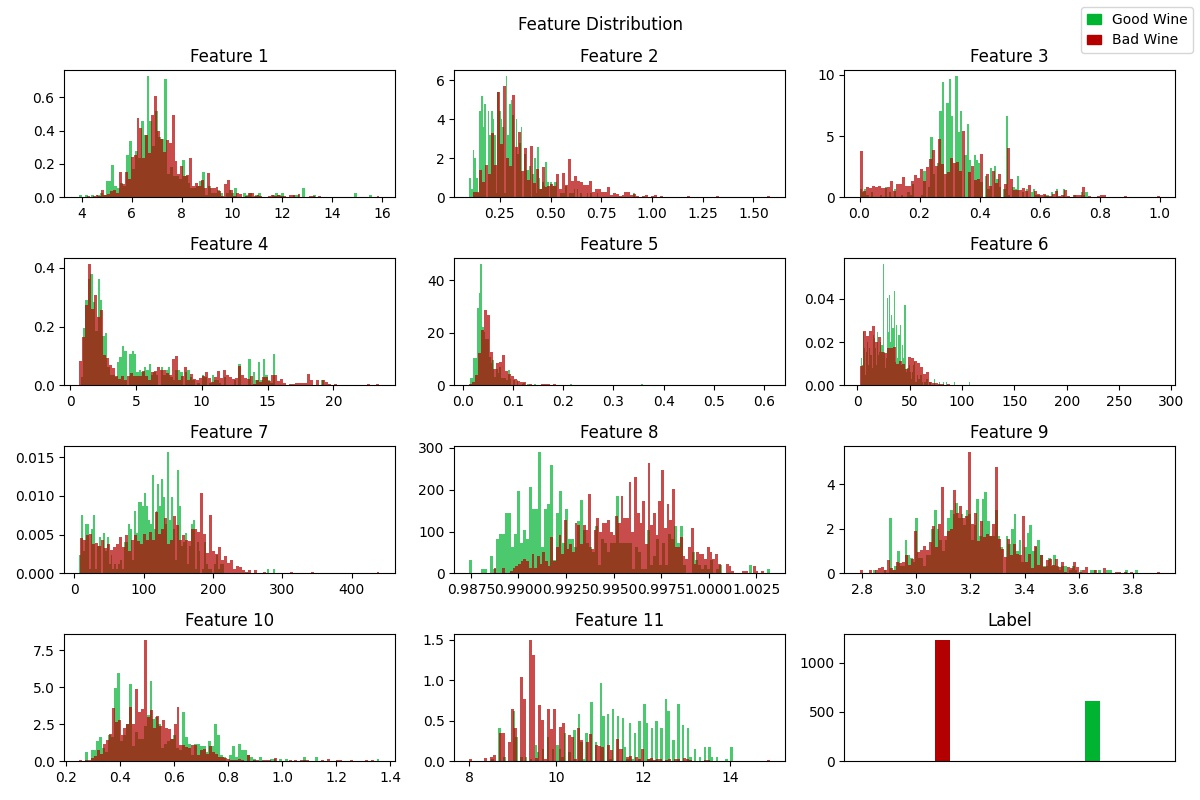
\includegraphics[width=\linewidth]{dist.jpg}}
    \label{featureshist}
\end{figure}

We start by noticing that the order of magnitude of some features can differ much from one another: for example, if we look at feature 5, it seems to span from 0.0 to as much as 0.6, but feature 7 instead spans two whole orders, occasionally being over 200, and with some outliers even double as much. An interesting observation is that some features do look gaussian distributed or regular enough to be described by a combination of gaussian distributions.

This may hint that some dimensionality reduction will be strongly biased towards features like 7, and that normalization can be taken as a valid pre-processing technique.

We also notice that our dataset is unbalanced: the quantity of bad wine is roughly twice the quantity of good one. This has to be taken into account when developing models, but we will be trating them as if the dataset is balanced, that is considering and equal probability of good wine and bad wine, occasionally rebalancing scores.

Let's apply a 2D projection of our data to further discuss it.

\begin{figure}[H]
    \caption{2D-PCA Projection}
    {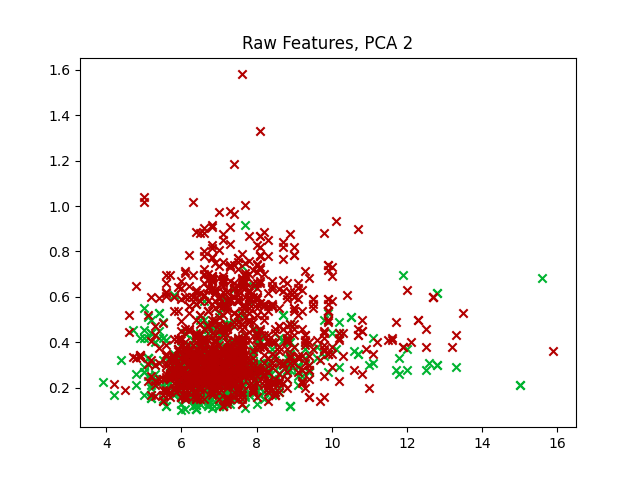
\includegraphics[width=\linewidth]{2DRAW.png}}
    \label{2DRAW}
\end{figure}

The features look highly correlated and fairly regularly distributed: this may be a hint that some gassuain models may perform well enough, like Full-Covariang MVG Classifiers or Tied-Covariance ones, but some other with linear decision boundaries, like linear SVMs, may perform poorly.

\begin{figure}[H]
    \caption{2D-PCA Projection, Normalized Data}
    {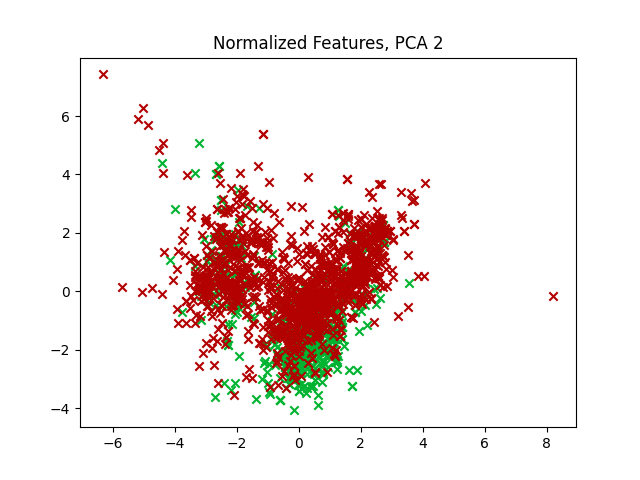
\includegraphics[width=\linewidth]{2DNorm.png}}
    \label{2DNORM}
\end{figure}

After normalization (Z-Normalization, mean $\mu = 0$ and St.D. $\sigma = 1$ ) our points do get apart but not significantly: we could expect linear models to still perform poorly and gaussian classifiers to get slightly worse. On the other hand, Gaussian Mixture Models look like a more interesting choice.

Lastly we take a look at normalized and whitened data.

\begin{figure}[H]
    \caption{2D-PCA Projection, Whitened Data}
    {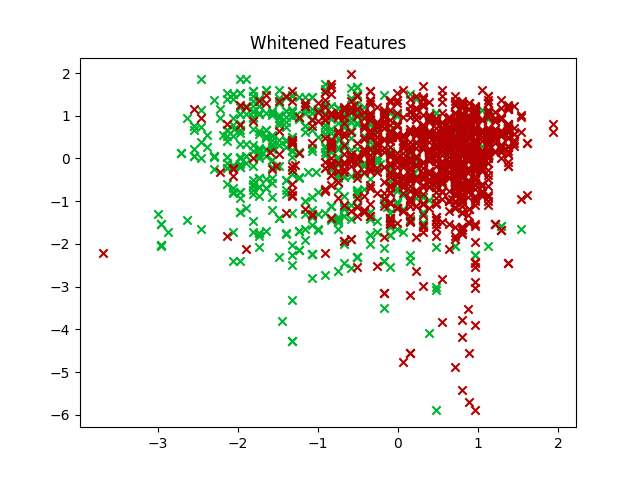
\includegraphics[width=\linewidth]{2DWhitened.png}}
    \label{2DWHI}
\end{figure}

Here the results are a bit more interesting: points do get separeted just like after normalization, but same class points stay close to each other while different class get more apart. In this scenario, it looks like even linear model might have a chance to achieve a decent performance.

\newpage
\section{Pre-Processing Analysis}
\subsection{Pre-Processing for Gaussian Models}

We will shortly decide, by running some non-optimized models, which pre-processing techniques are useful and which are not. 

We will be reporting the best results for each classifiers, extracted from a 3 or 5 Fold Validation approach. The decision rule, since this is a binary problem, will be set to $\displaystyle t = \log(\frac{\pi_T}{1-\pi_T}) \lessgtr 0 $, where $\pi_T$ is assumed $ = 0.5$ and it is the prior probability of class Good.

Let's start with Gaussian Classifiers: Full-Covariance, Tied-Covariance, and Naive-Bayes.
We find out that a small number of features can be removed, with modest gains.

Let's combine these results with normalization and whitening.

\begin{table}[H]
    \centering
        \begin{tabular}{||c|c|c|c||}
            \hline
            Type & PCA & DCF & minDCF \\
            \hline
            \hline
            Raw & 9 & 0.401 & {\bf 0.362}  \\
            Normalized &  7 & 0.464 & 0.420 \\
            Whitened & 2 & 0.430 & 0.410 \\
            \hline
    \end{tabular}
    \caption{Full-Covariance MVG - Best Results}
\end{table}

\begin{table}[H]
    \centering
        \begin{tabular}{||c|c|c|c||}
            \hline
            Type & PCA & DCF & minDCF \\
            \hline
            \hline
            Raw & 7 & {\bf 0.375} & 0.366  \\
            Normalized &  9 & {\bf 0.375} & 0.371 \\
            Whitened & 11 & 0.402 & 0.401 \\
            \hline
    \end{tabular}
    \caption{Tied-Covariance MVG - Best Results}
\end{table}

\begin{table}[H]
    \centering
        \begin{tabular}{||c|c|c|c||}
            \hline
            Type & PCA & DCF & minDCF \\
            \hline
            \hline
            Raw & 7 & 0.383 & 0.366  \\
            Normalized &  10 & 0.429 & 0.391 \\
            Whitened & 5 & 0.402 & 0.386 \\
            \hline
    \end{tabular}
    \caption{Naive-Bayes MVG - Best Results}
\end{table}

Now we can finally say something on MVG Classifiers:

\begin{itemize}
    \item As expected, the Tied Covariance model works fairly well
    \item Unexpectedly, the Naive-Bayes model outperforms the Full-Covariance one, even without whitening
    \item Normalization and whitening seem to hurt performance
    \item PCA can be used, but gains are not particularly high
\end{itemize}

\subsection{Pre-Processing for GM Models}

Staying of the subject of Gaussian Classifiers, we make similar operations for GMMs. 
This is a dummy 4-Component model.

Results seem on par, not significantly lower than MVG Classifiers, but GMM actually performs best when keeping as much dimensions as possible.

\begin{table}[H]
    \centering
        \begin{tabular}{||c|c|c|c||}
            \hline
            Type & PCA & DCF & minDCF \\
            \hline
            \hline
            Raw & No & 0.410 & {\bf 0.394}  \\
            Normalized &  9 & {\bf 0.407} & 0.402 \\
            Whitened & 4 & 0.429 & 0.420 \\
            \hline
    \end{tabular}
    \caption{GMM - Best Results}
\end{table}

Also here, normalization and whitening seem to do more bad than good. Results do not get much worse, sometimes even get better but not significantly.

Our best option is to work with raw features on GMMs. Weirdly enough, Whitened GMM can discard many components and still perform fairly well compared to the raw counterpart.


In the next two subsections we will discuss pre-processing on two types of kernel SVMs: Polynomial and RBF ones. 
Given the non-probabilistic nature of the scores, using a threshold of $0$ is somewhat an arbitrary choice: to account for that, we will be giving a greater importance to minimum DCFs rather than plain DCFs.

\subsection{Pre-Processing for Polynomial Kernel SVMs}

As usual we start by looking at the effect of PCA on a dummy Polynomial Kernel. The dummy kernel used is the following:

$$ \phi({\bf x}_1)^T\phi({\bf x}_2) = k({\bf x_1}, {\bf x_2}) = $$
$$ = ({\bf x}_1^T{\bf x}_2 + c)^d + b = ({\bf x}_1^T{\bf x}_2+1)^2+0.5$$

With $\phi(\cdot)$ being:

\begin{center}
    \begin{align}
        \phi({\bf x}) & = \begin{bmatrix}
                            vec({\bf x}{\bf x}^T) \\
                            \sqrt{2}{\bf x} \\
                            1 \\
                      \end{bmatrix}
    \end{align}
\end{center}
\footnote{Above we freely set $c$ as it is the final derivation of this mapping, but the original kernel as desccribed here would require it to be 1}

Generally speaking, results look far from good ( the DCFs are much higher than Gaussian Models ) and PCA seems to have no effect whatsoever.

\begin{table}[H]
    \centering
        \begin{tabular}{||c|c|c|c||}
            \hline
            Type & PCA & DCF & minDCF \\
            \hline
            \hline
            Raw & 11 & 0.648 &  0.642 \\
            Normalized & 10 & 0.666 &  0.653 \\
            Whitened & 11 & 0.666 &  0.659 \\
            \hline
    \end{tabular}
    \caption{Polynomail Kernel SVM - Best Results}
\end{table}

Here normalization and whiteining seem to have little to no effect: our DCFs are the same, even thought our scores vary significantly.

Moreover, since we are enforcing $\pi_T = 0.5$, this means that we are achieving $ \approx 33\% $ error rate, which is the same we would get by guessing always Bad (on our Training/Validation set, that is).
This may hint that polynomial kernel SVMs are just bad suited for this task.

\subsection{Pre-Processing for RBF Kernel SVMs}

Just like we did for the polynomial one, here we try again a dummy kernel to see how we should pre-process our data.
The dummy kernel function used is: 

$$\displaystyle k({\bf x_1}, {\bf x_2}) = e^{-\gamma||{\bf x}_1 - {\bf x}_2||^2} + b = e^{-0.05||{\bf x}_1 - {\bf x}_2||^2} + 0.05 $$

Small values of $\gamma$ and $b$ were picked to avoid numerical issues.

The RBF seems to be robust while working with all features or almost, and start behaving worse when the number of dimensions gets much lower.

Given the non-optimed hyperparameters, trying various combination of hyperparameters with high dimensionalities is needed to draw any conclusions.

\begin{table}[H]
    \centering
        \begin{tabular}{||c|c|c|c||}
            \hline
            Type & PCA & DCF & minDCF \\
            \hline
            \hline
                Raw & 10 & 0.585 &  0.579 \\ 
                Normalized & No &  {\bf 0.469}  &  {\bf 0.431} \\
                Whitened & No &  {\bf 0.469}  &  {\bf 0.431} \\
            \hline
    \end{tabular}
    \caption{RBF Kernel SVM - Best Results}
\end{table}

For once normalization seems to help: the DCFs get significantly lower. 
Whitened features perform on par with normalized features, but given that before whiteining features are also normalized, we can say that also in this case whiteining has no effect whatsoever.

\newpage
\section{Optimizing Models}
\subsection{Optimizing MVG Classifiers}

\end{document}